% \includegraphics{IMG_2840.JPG}

\begin{figure}[H]
	\centering
	\begin{minipage}{0.4\textwidth}
	\centering
	\includegraphics[angle=90,width=1.0\textwidth]{IMG_2840.JPG}
	\caption{The right hand}
	\label{fig:right_hand_position}
	\end{minipage}
	\hfill
	\begin{minipage}{0.4\textwidth}
	\centering
	\vspace{1cm}
	\includegraphics[angle=90,width=1.0\textwidth]{IMG_2845.JPG}
	\caption{The left hand}
	\label{fig:left_hand_position}
	\end{minipage}
	\\
	\centering
	\begin{minipage}{0.4\textwidth}
	\centering
	\includegraphics[angle=90,width=1.0\textwidth]{IMG_2842.JPG}
	\caption{The angle}
	\label{fig:angle}
	\end{minipage}
	\hfill*

\end{figure}

\begin{figure}[H]
	\centering
	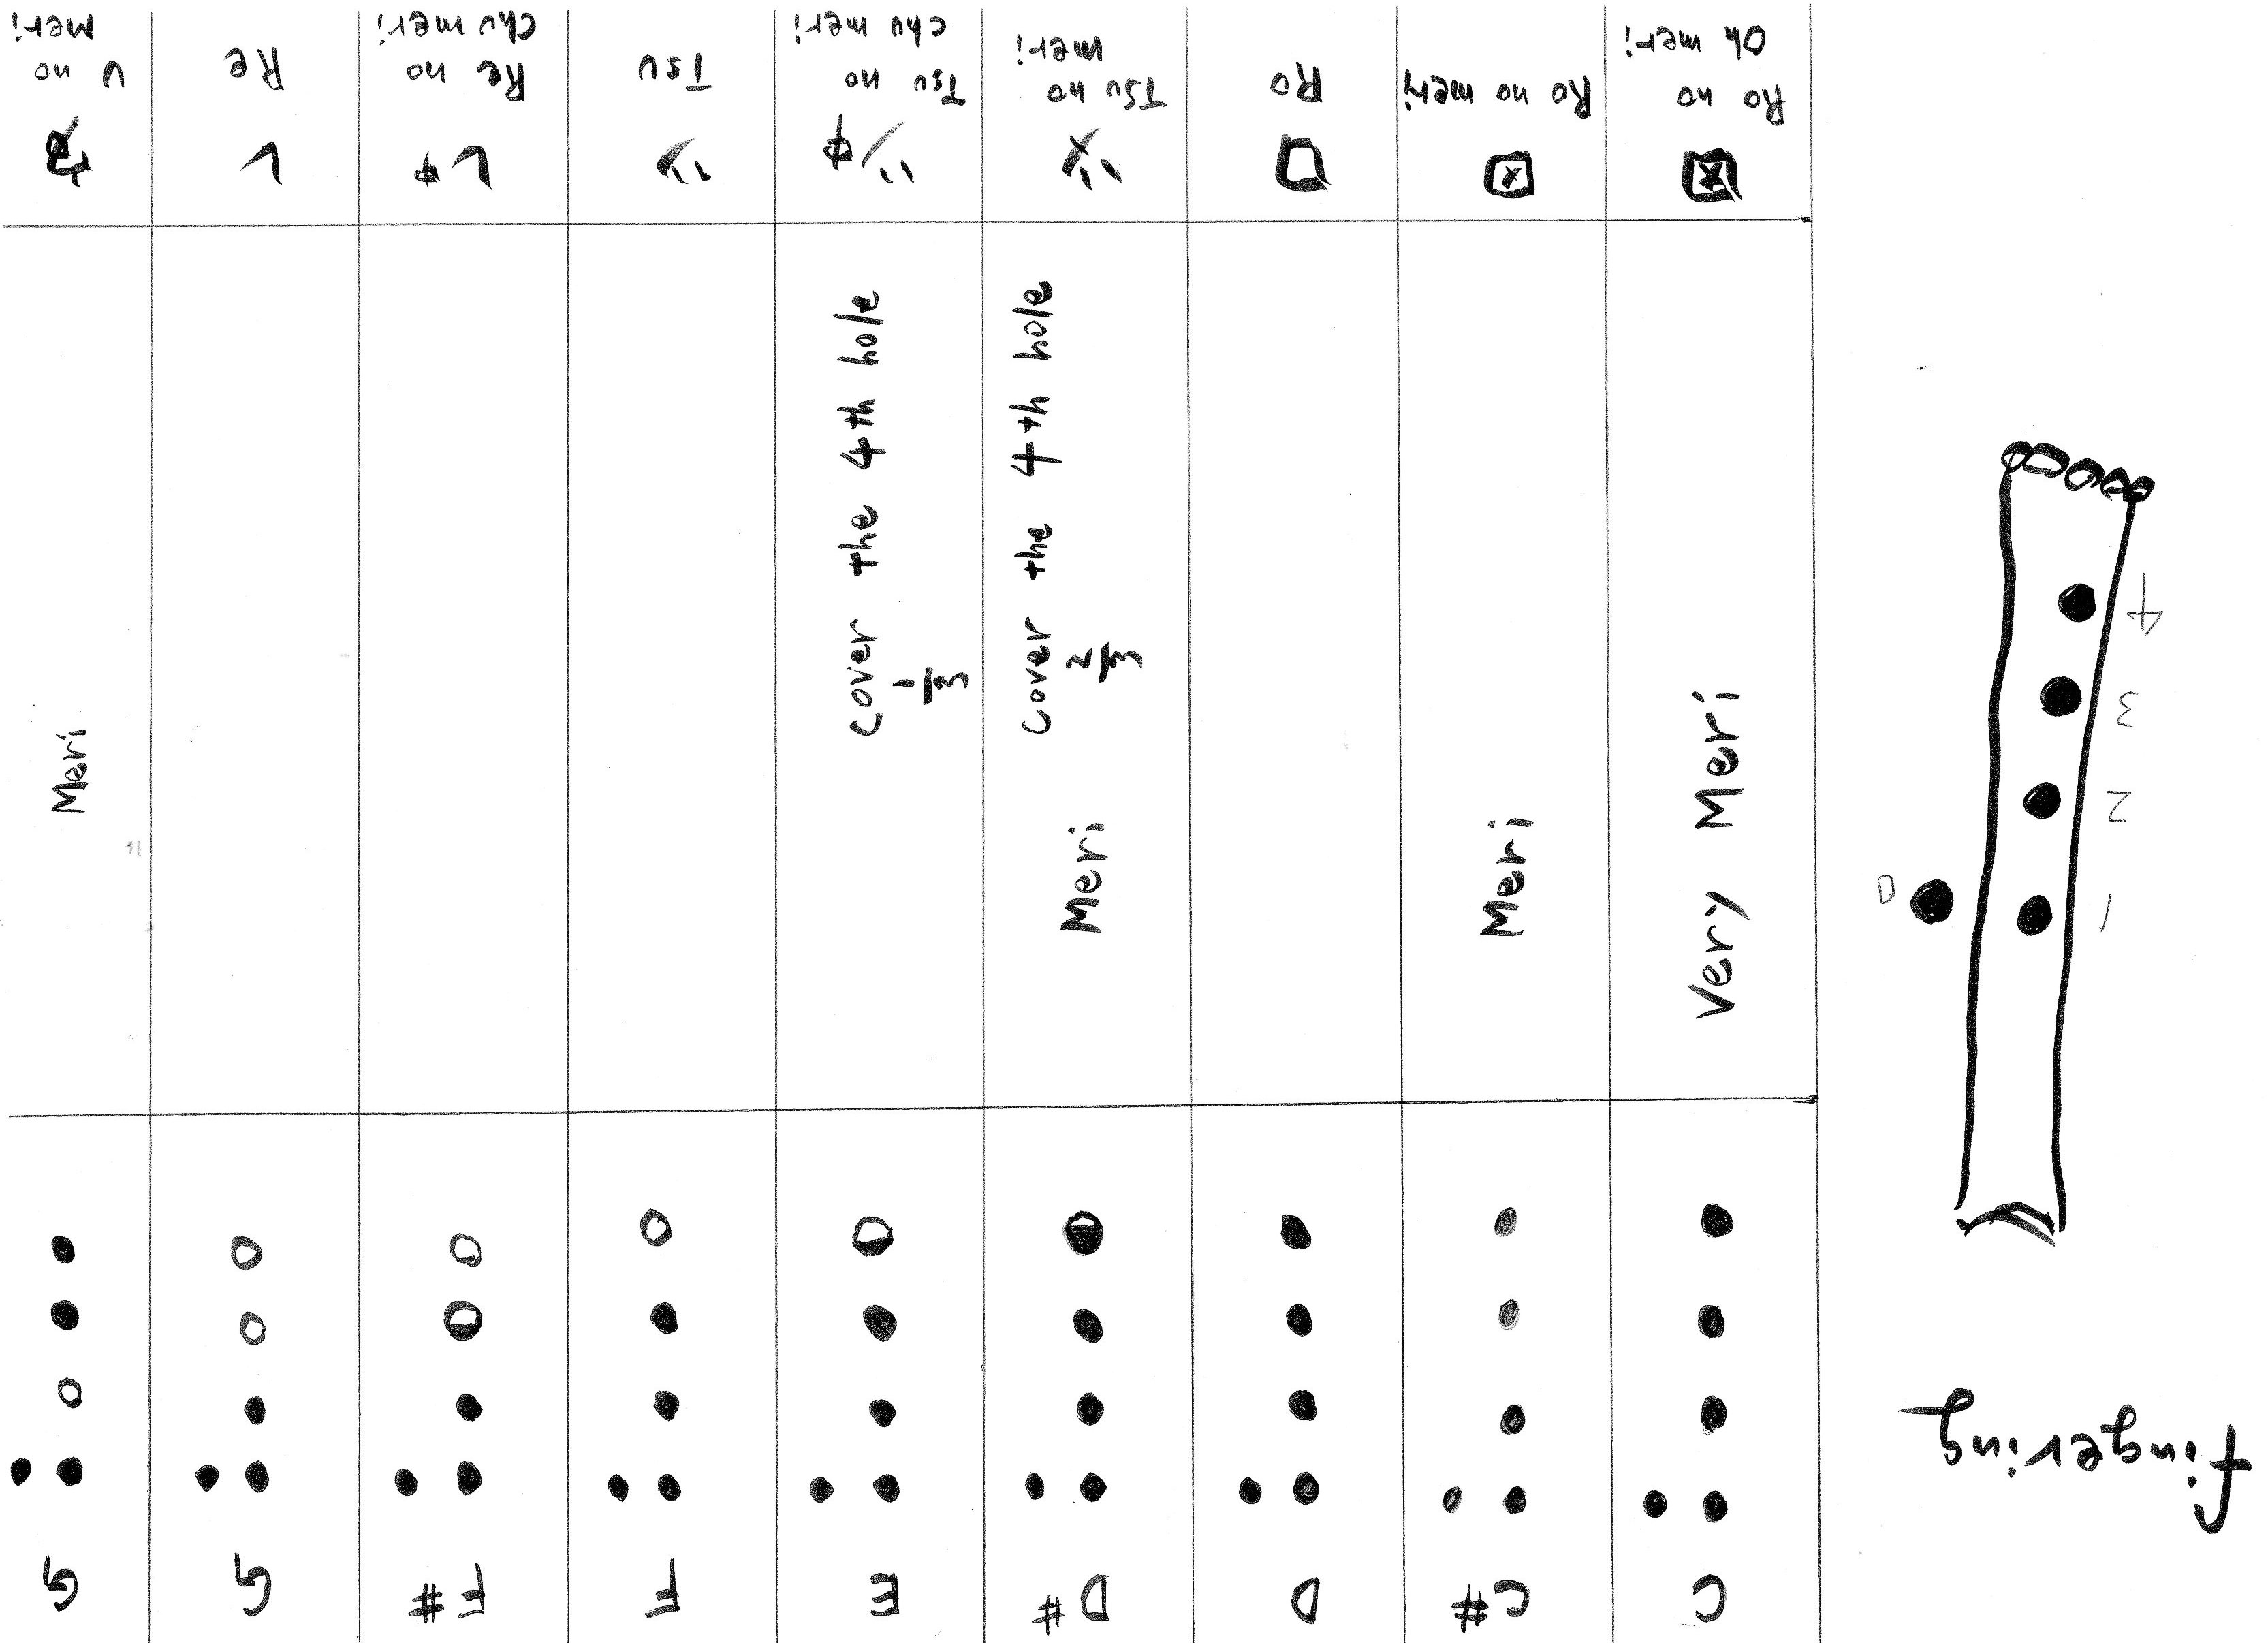
\includegraphics[angle=0,width=1.0\textwidth]{尺八の運指表1}
	\caption{Shakuhachi fingerings Part 1}
	\label{fig:shakuhachi_fingerings_1}
\end{figure}

\begin{figure}[H]
	\centering
	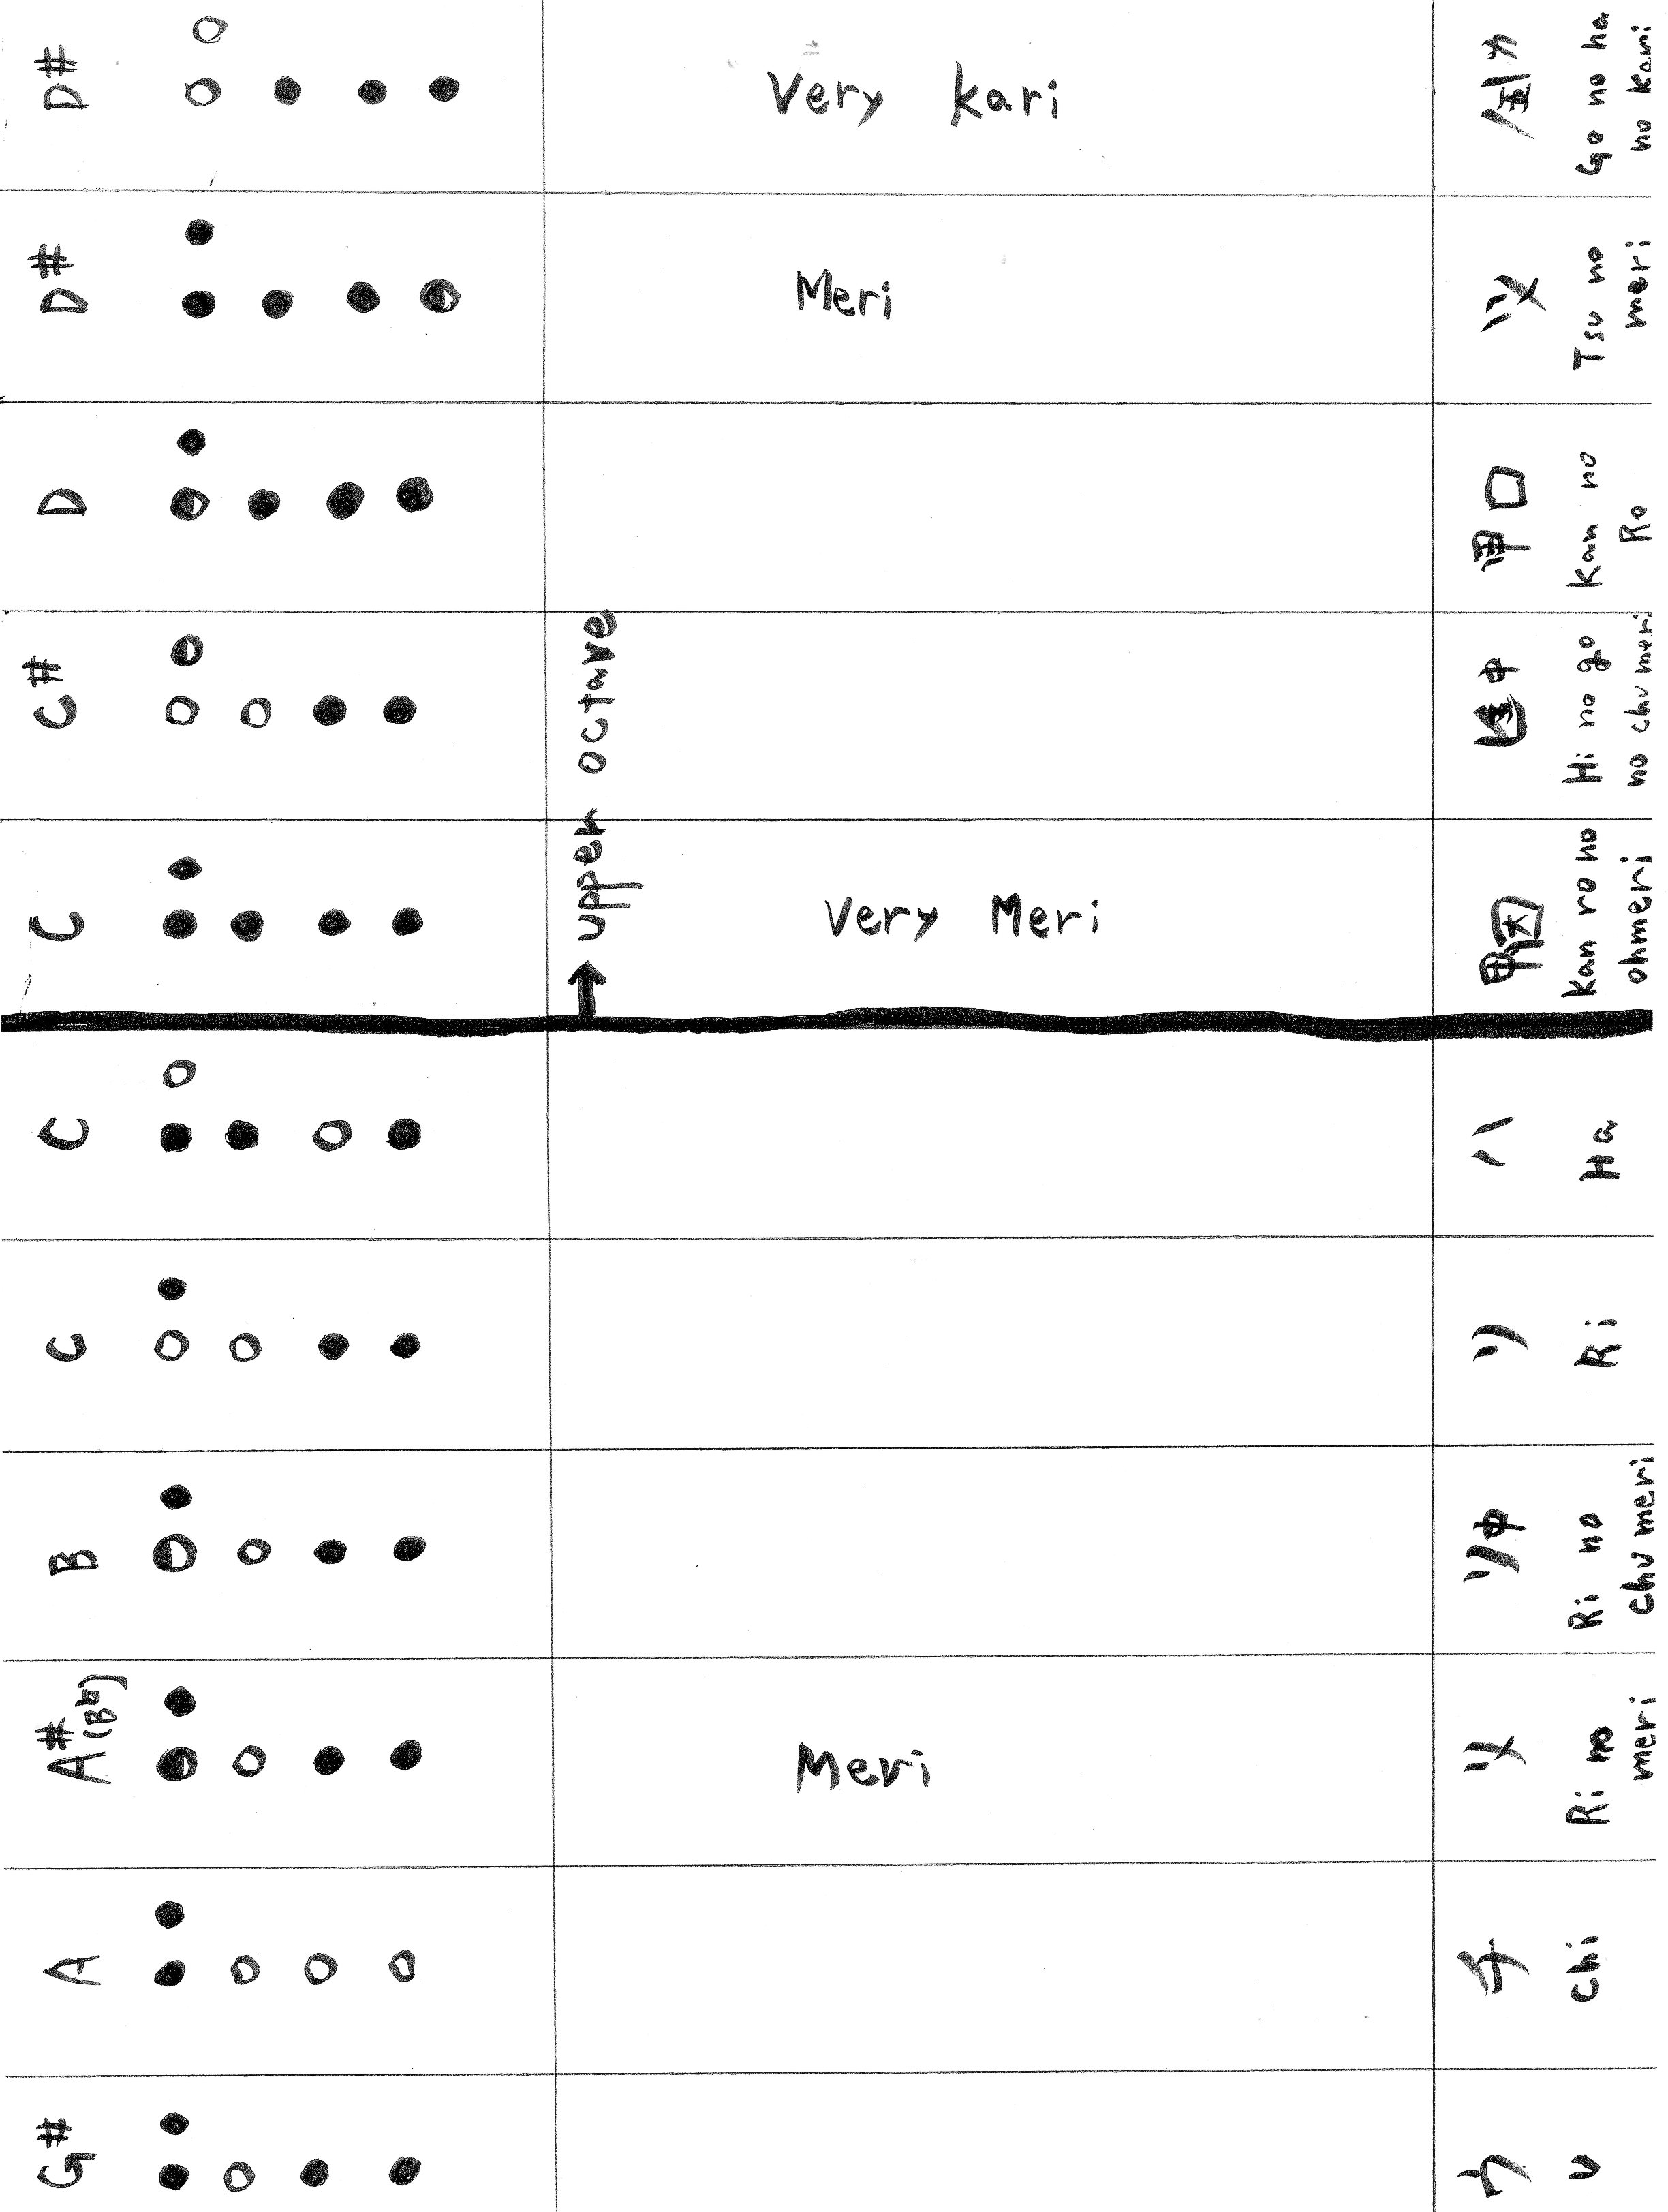
\includegraphics[angle=0,width=1.0\textwidth]{尺八の運指表2}
	\caption{Shakuhachi fingerings Part 2}
	\label{fig:shakuhachi_fingerings_2}
\end{figure}

\begin{figure}[H]
	\centering
	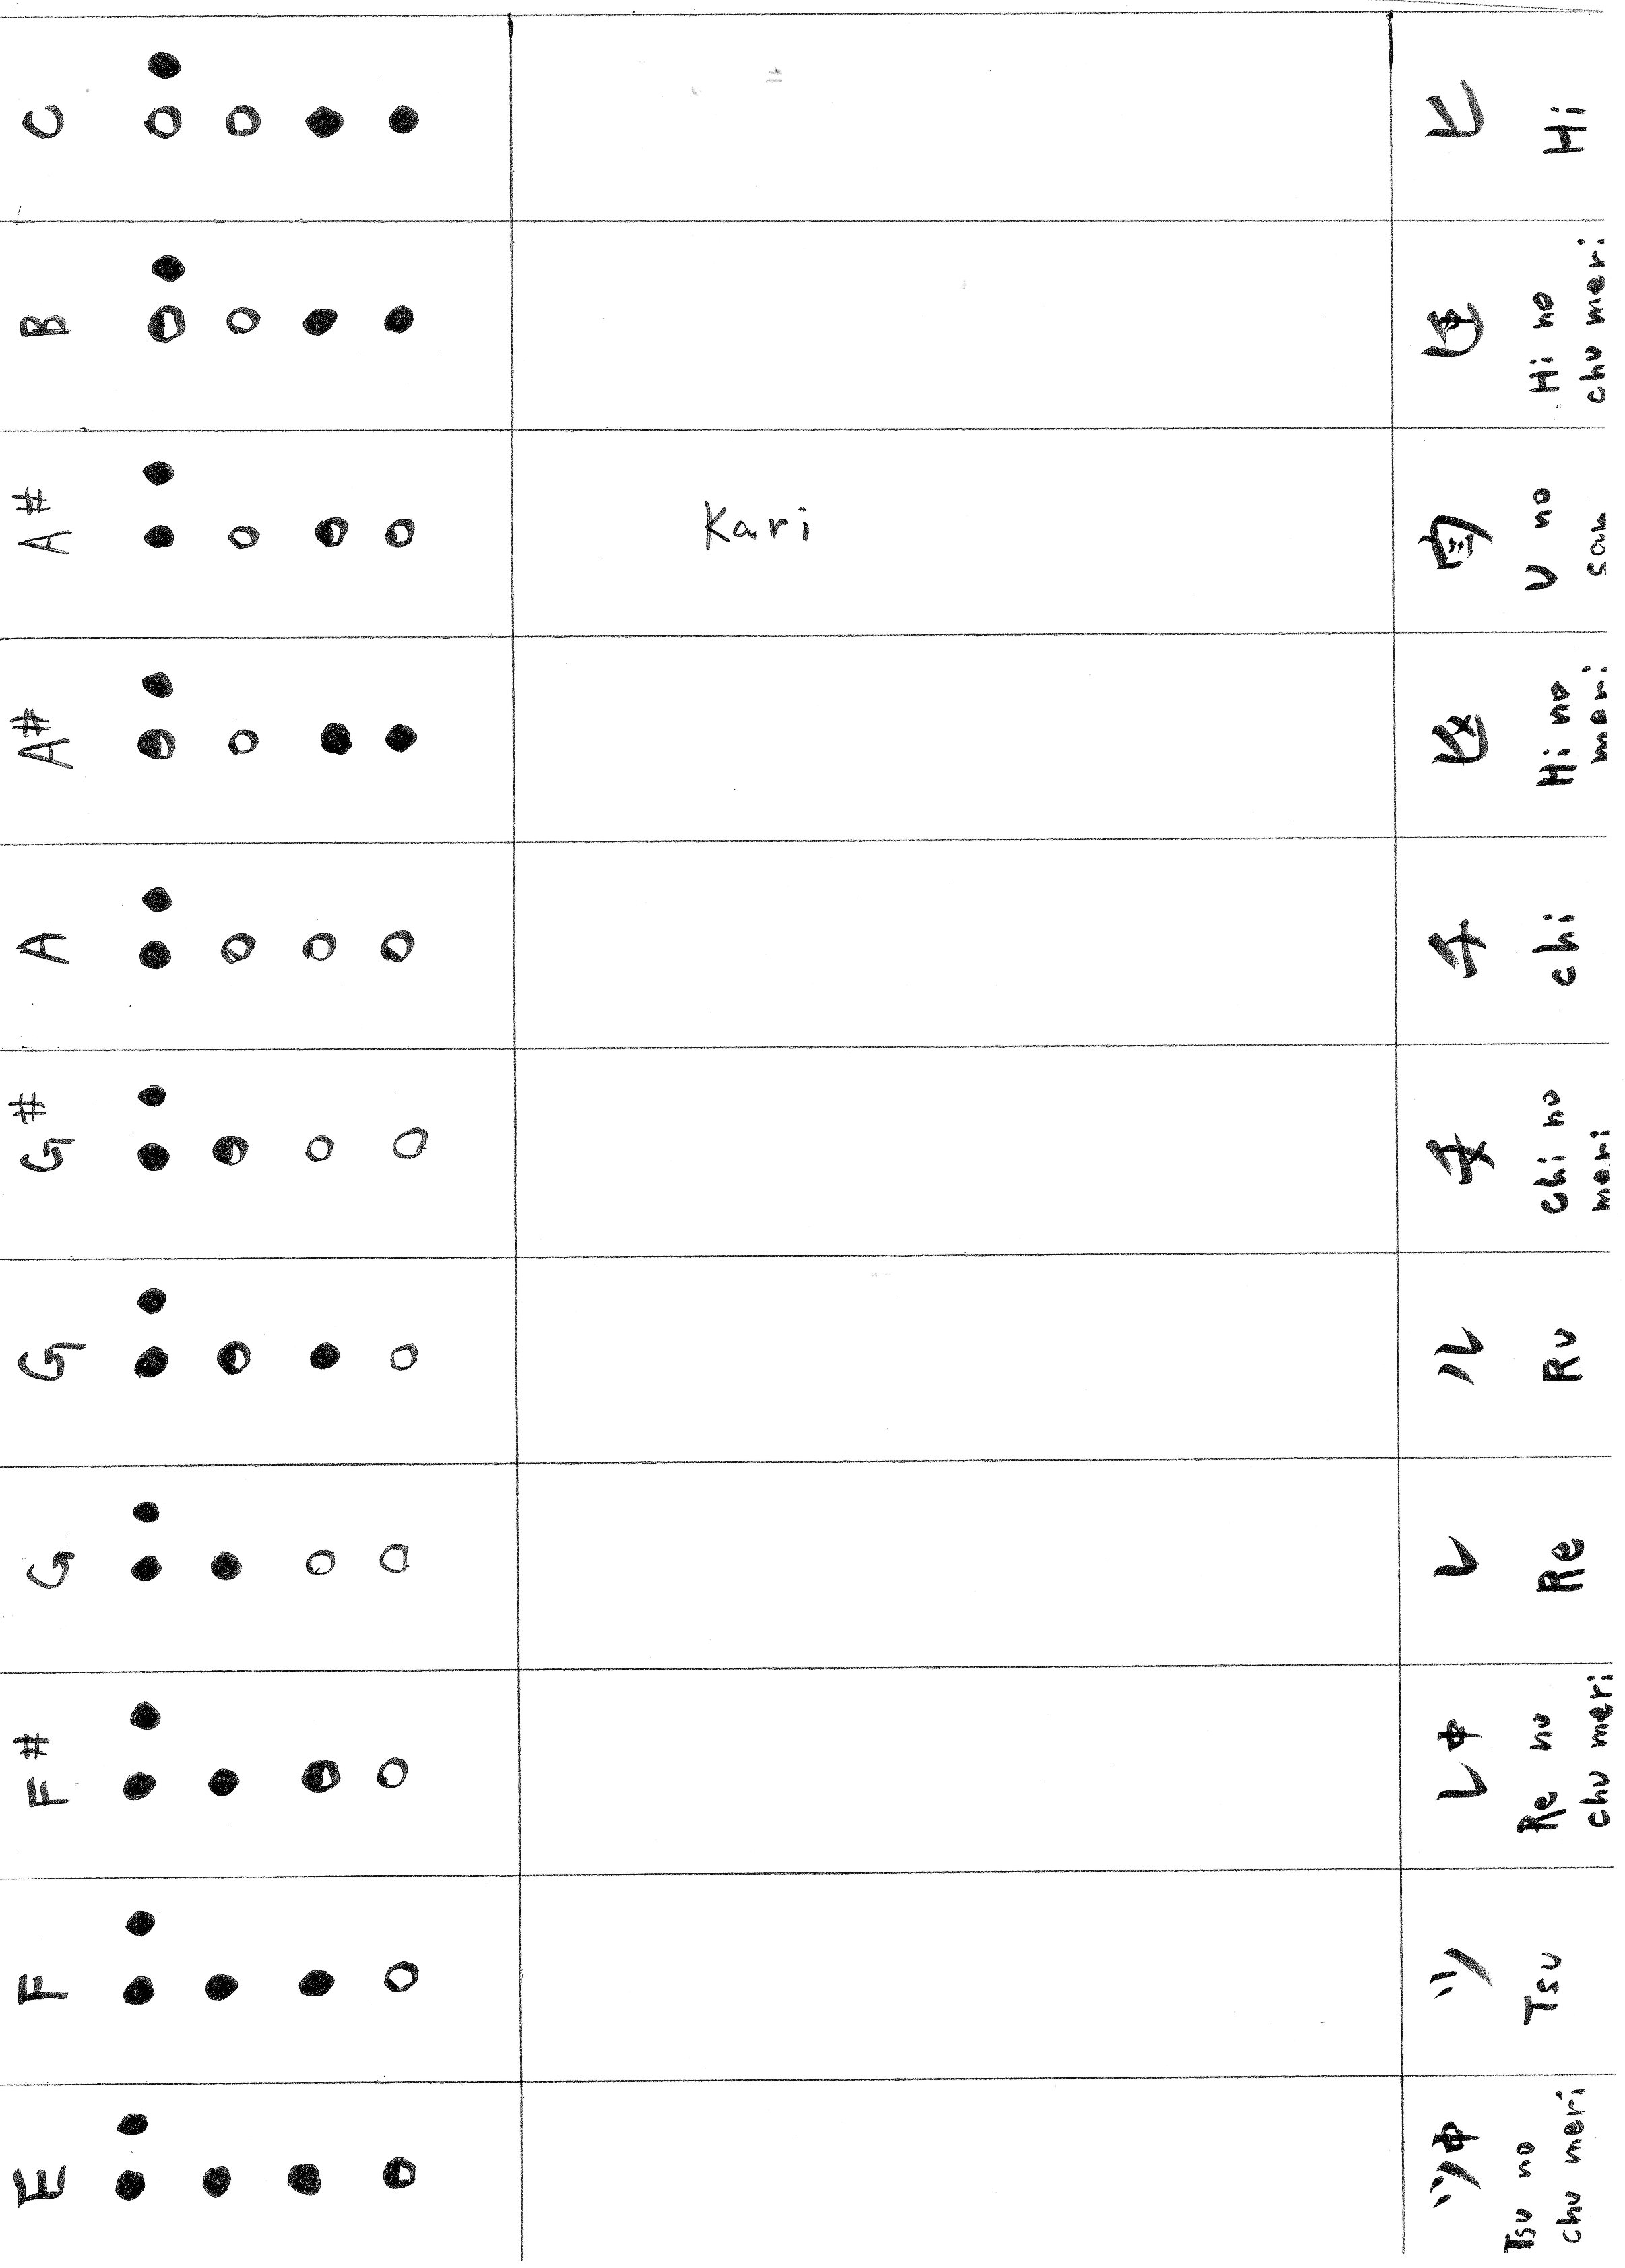
\includegraphics[angle=0,width=1.0\textwidth]{尺八の運指表3}
	\caption{Shakuhachi fingerings Part 3}
	\label{fig:shakuhachi_fingerings_3}
\end{figure}

\begin{figure}[H]
	\centering
	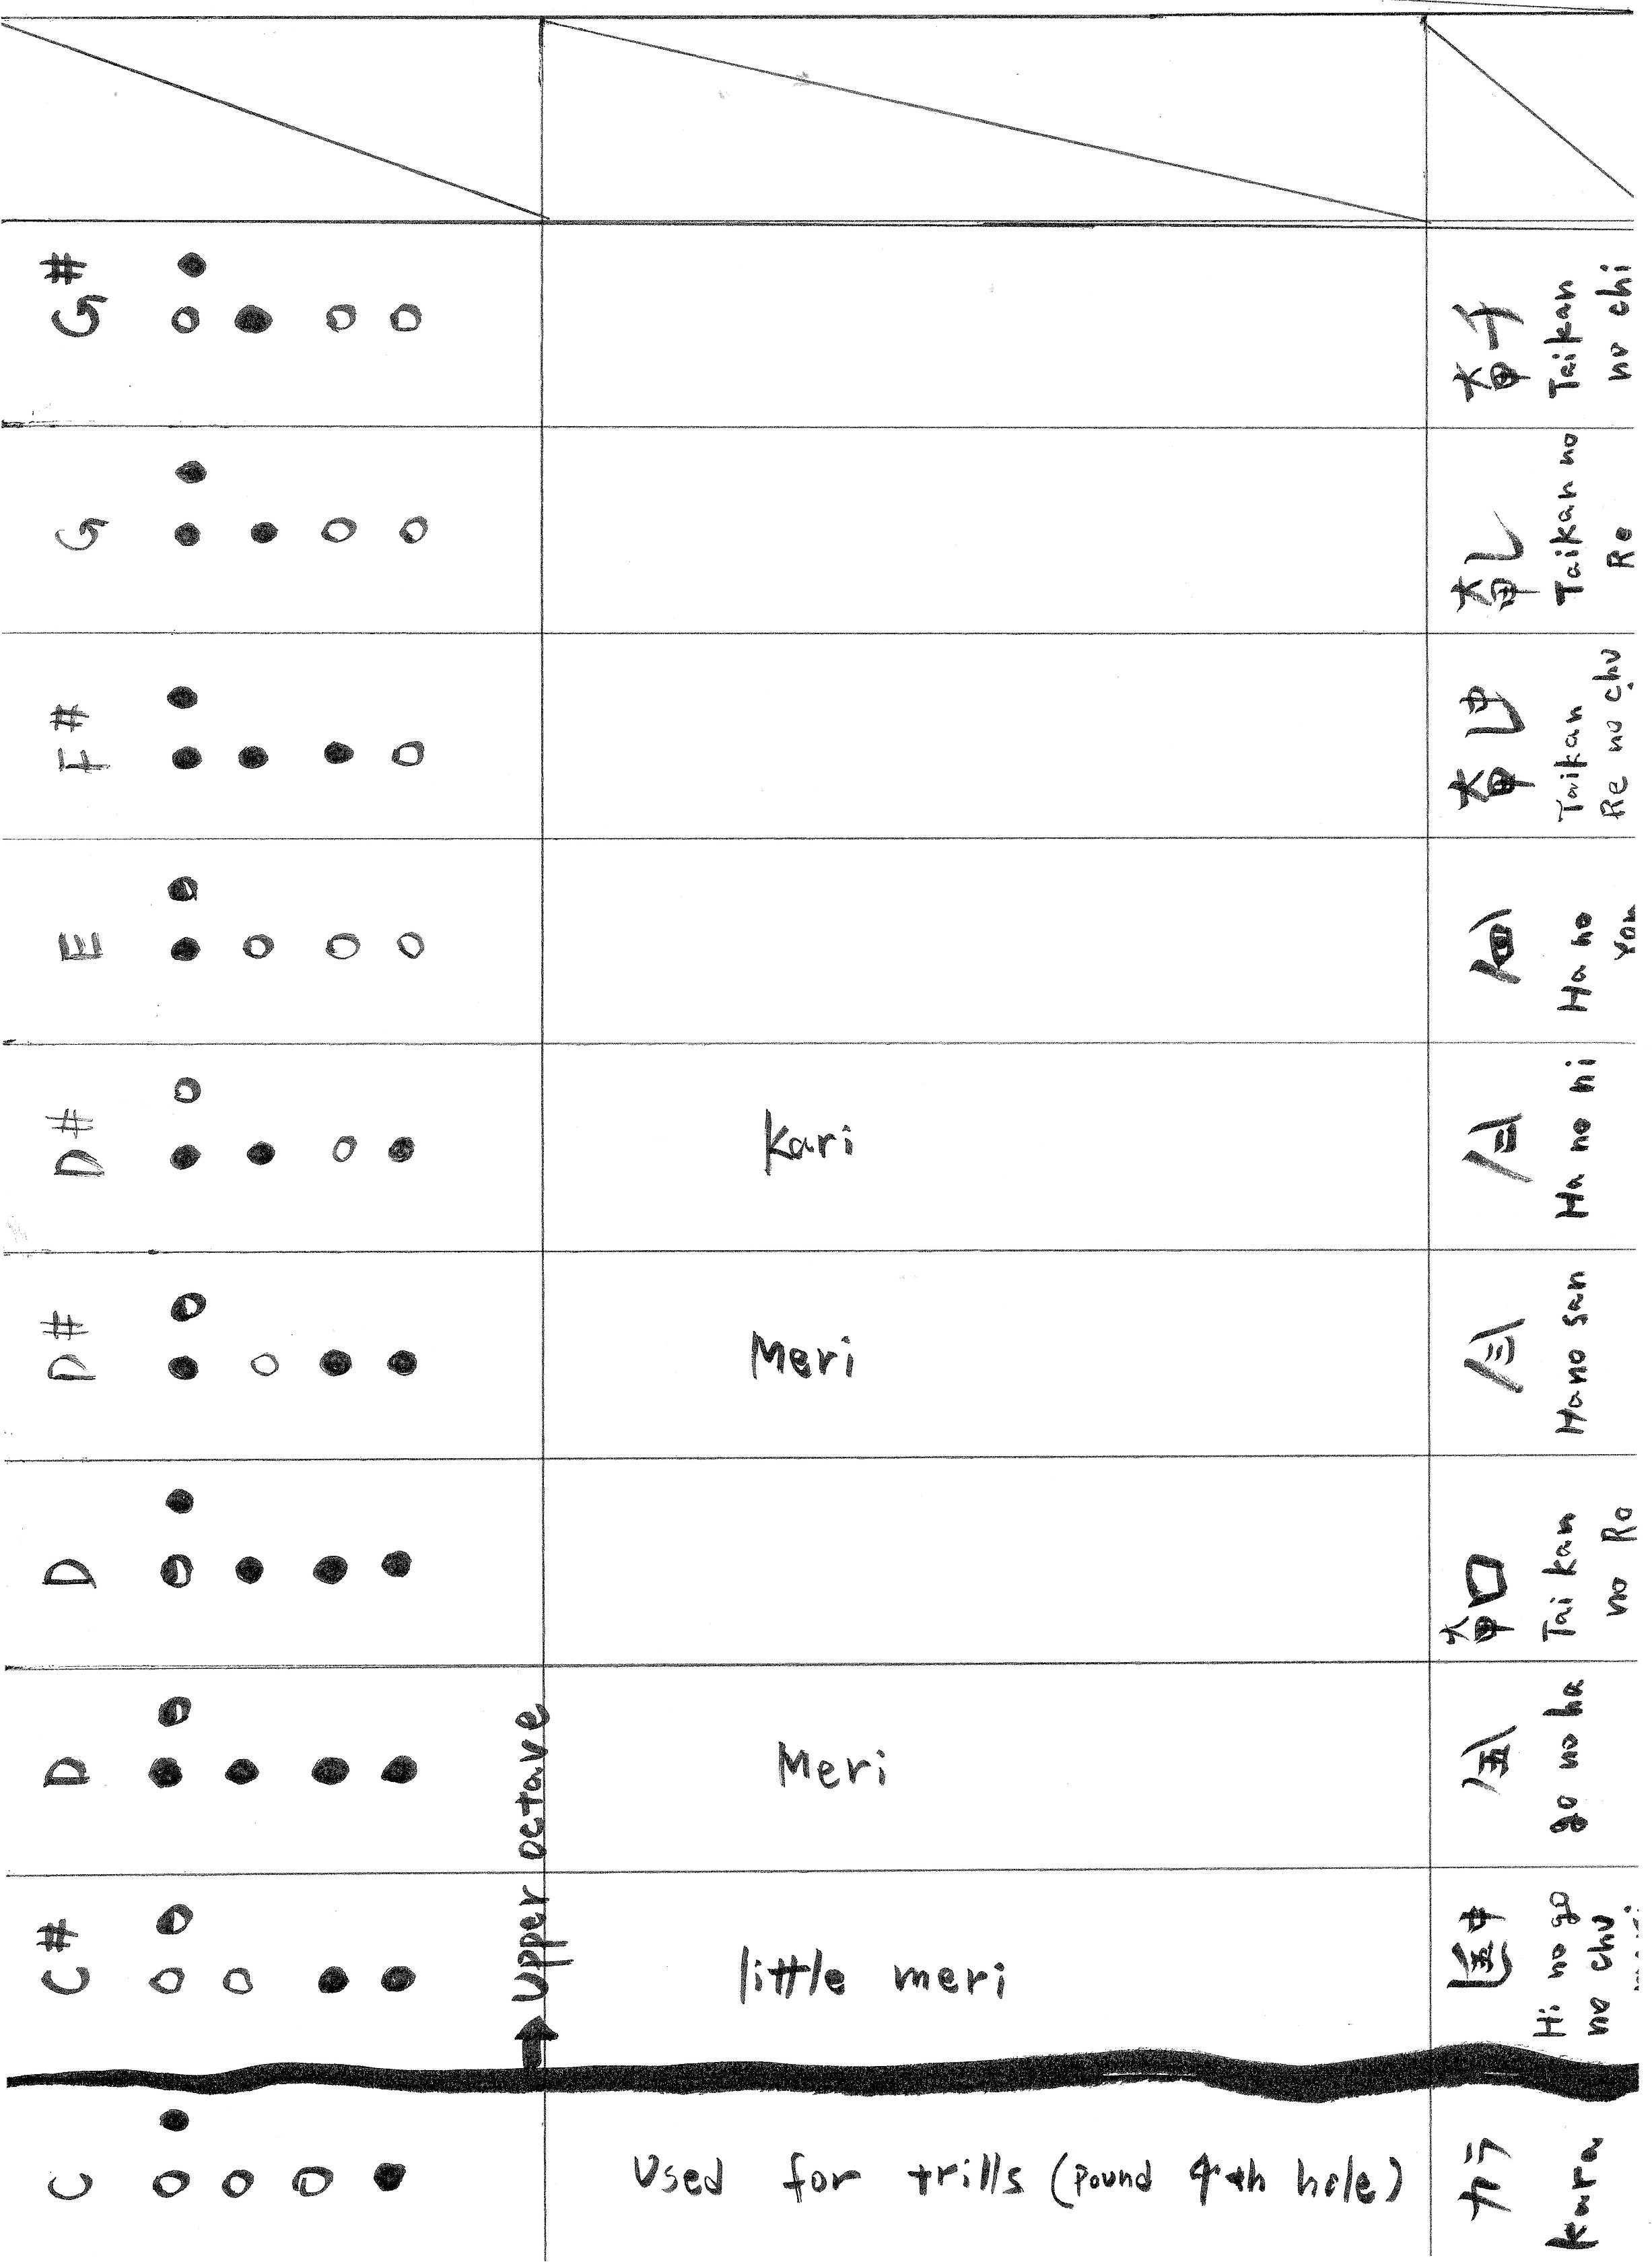
\includegraphics[angle=0,width=1.0\textwidth]{尺八の運指表4}
	\caption{Shakuhachi fingerings Part 4}
	\label{fig:shakuhachi_fingerings_4}
\end{figure}

\vfill

\begin{figure}
	\centering
	\begin{minipage}{0.9\textwidth}
	\centering
	\includegraphics[angle=0,width=0.75\textwidth]{halfhole.pdf}
	\caption{Half-holing} \label{fig:half-holing}
	\includegraphics[angle=0,width=0.75\textwidth]{pinch.pdf}
	\caption{Pinching} \label{fig:pinching}
	\end{minipage}
\end{figure}
